\documentclass[12pt]{article}
\usepackage[a4paper,margin=1in]{geometry}
\usepackage{amsmath,amssymb,amsfonts}
\usepackage{graphicx}
\usepackage{booktabs}
\usepackage{siunitx}
\usepackage{titlesec}
\usepackage{caption}
\usepackage{longtable}
\usepackage{fancyhdr}
\usepackage{enumitem}
\usepackage{float}
\usepackage{etoolbox}
\usepackage{xurl}
\usepackage{adjustbox}
\usepackage{microtype}
\usepackage{natbib}
\usepackage{listings}
\usepackage{upquote}
\usepackage{xcolor}
% Preamble (if not already there)
\usepackage{tikz}
\usetikzlibrary{arrows.meta, positioning, shapes.geometric}
\usepackage{lscape}
\usepackage[colorlinks=true,
            linkcolor=blue,
            citecolor=blue,
            filecolor=blue,
            urlcolor=blue]{hyperref}

% --- Notation patch (hsB--SM) ---
% Slopes: use \iota (not \gamma, which is psychrometric)
\newcommand{\slope}{\iota}
% Psychrometric constant:
\newcommand{\gpsy}{\gamma_{\mathrm{psy}}}
% von Kármán constant:
\newcommand{\karm}{\kappa}
% Infiltration capacity:
\newcommand{\fcap}{f_{\mathrm{cap}}}
% Channel width function (pdf of flow path lengths):
\newcommand{\omegac}{\omega_c}
% Unit hydrograph (routing):
\newcommand{\UH}{u_c}

% Setup spacing and styles
\setlength{\parskip}{0.8em}
\setlength{\parindent}{0pt}
\sisetup{detect-all, output-exponent-marker=\ensuremath{\mathrm{e}}, per-mode=symbol}

% Header/Footer
\pagestyle{fancy}
\fancyhf{}
\rhead{1D hsB - SM Model}
\lhead{Marcus N. Gomes Jr., Ph.D.}
\cfoot{\thepage}

% Title setup
\title{\textbf{Coupled Surface-Subsurface Hillslope Hydrological Model: hsB--SM Model: MATLAB Formulation and Python Implementation}}
\author{Marcus Nóbrega Gomes Jr.}
\date{Python version 0.1.0, documentation revised 25 November 2026}

\lstset{basicstyle=\ttfamily\small,breaklines=true,breakatwhitespace=false,
 columns=fullflexible,keepspaces=true,showstringspaces=false,upquote=true,frame=single,
 rulecolor=\color{gray!35},xleftmargin=0.3em,xrightmargin=0.3em}
\setlength{\headheight}{16pt}
\emergencystretch=2em
\AtBeginEnvironment{tabular}{\small}
\begin{document}

\maketitle
\tableofcontents
\newpage

% ------------------------------
\section*{Author Information}
\addcontentsline{toc}{section}{Author Information}

\textbf{Marcus N. Gomes Jr.} \\
Ph.D. - Postdoctoral Researcher II at University of Arizona \\

\vspace{0.5em}

\begin{adjustbox}{max width=\linewidth}\begin{tabular}{ll}
\textbf{Website:} & \href{https://marcusnobrega-eng.github.io/profile/}{\texttt{marcusnobrega-eng.github.io/profile}} \\
\textbf{C.V.:} & \href{https://marcusnobrega-eng.github.io/profile//files/CV___Marcus_N__Gomes_Jr_.pdf}{\texttt{CV}} \\
\textbf{ORCID:} & \href{https://orcid.org/0000-0002-8250-8195}{\texttt{https://orcid.org/0000-0002-8250-8195}} \\
\textbf{GitHub:} & \href{https://github.com/marcusnobrega-eng}{\texttt{https://github.com/marcusnobrega-eng}} \\
\textbf{Email:} & \texttt{marcusnobrega.engcivil@gmail.com}
\end{tabular}\end{adjustbox}

\newpage
% ----------------------------------------------------------------
\section{Quick Start: Configuring Your First Model}
\label{sec:python_quickstart}

This section describes how to install hsB--SM, prepare catchment inputs, set the parameters and initial conditions, and run the model. A forward simulation requires hillslope geometry, a channel travel-distance distribution, and meteorological time series. Observed discharge is optional for simulation and is needed for evaluation or calibration. The equations and implementation details follow in the later sections.

\subsection{Install the model}

Install Python 3.11 or newer and Git. Open a terminal and download the Python repository.

\begin{lstlisting}[language={},caption={Download the repository.}]
git clone https://github.com/mariaandradeal/1D_hsb-SM-python.git
cd 1D_hsb-SM-python
\end{lstlisting}

On Windows PowerShell, create and activate a Python environment, then install the package.

\begin{lstlisting}[language={},caption={Install on Windows.}]
python -m venv .venv
.\.venv\Scripts\Activate.ps1
python -m pip install -e .
\end{lstlisting}

If PowerShell blocks activation, use \path{.\.venv\Scripts\python.exe} in place of \texttt{python} in the installation and model commands. Activation is optional.

On macOS or Linux, use the following commands.

\begin{lstlisting}[language={},caption={Install on macOS or Linux.}]
python3 -m venv .venv
source .venv/bin/activate
python -m pip install -e .
\end{lstlisting}

\subsection{Prepare the input files}

From the repository root, copy \path{templates/catchment} to a new model directory. The copy command requires a new destination and does not overwrite an existing model. The CSV templates contain column headers only. Fill them with data for your catchment.

\begin{lstlisting}[language={},basicstyle=\ttfamily\footnotesize,caption={Create a model directory from the input template.}]
python -c "from shutil import copytree; copytree('templates/catchment', 'my_model')"
\end{lstlisting}

The model directory contains four input files. \path{geometry.csv} defines the hillslope cells, \path{channel.csv} defines the channel travel-distance distribution, \path{forcing.csv} contains meteorological and vegetation inputs, and \path{config.json} stores paths, the timestep, slopes, parameters, and initial conditions. Paths inside the configuration are relative to its directory.

In \path{geometry.csv}, supply cell-center distance \texttt{x\_m}, planform width \texttt{w\_m}, and cell length \texttt{dx\_m}, all in metres. Order cells from the outlet toward the divide. Distances, widths, and lengths must be positive. Each center must lie inside the cell edges obtained by accumulating cell lengths from the outlet. Supply prepared geometry tables; the Python package does not delineate a catchment from a digital elevation model.

In \path{channel.csv}, supply increasing positive channel distances \texttt{distance\_m} [m] and nonnegative bin weights \texttt{weight}. Their sum must be positive. The model normalizes the weights. For unequal distance-bin widths, use integrated probability masses.

The meteorological table has one row per forcing interval and the columns listed below. The forcing is spatially uniform across the hillslope.

{\small
\begin{longtable}{p{0.27\linewidth}p{0.62\linewidth}}
\toprule
Column & Meaning and unit \\
\midrule
\endhead
\texttt{date} & Start of the interval, as \texttt{YYYY-MM-DD} or \texttt{YYYY-MM-DD HH:MM:SS} \\
\texttt{P} & Precipitation rate [m\,s$^{-1}$] \\
\texttt{Temp\_C} & Air temperature [$^\circ$C] \\
\texttt{Pres\_kPa}, \texttt{VapP\_kPa} & Air pressure and actual vapor pressure [kPa] \\
\texttt{Wind\_ms} & Wind speed [m\,s$^{-1}$] \\
\texttt{SRad\_Wm2}, \texttt{LRad\_Wm2} & Incoming shortwave and longwave radiation [W\,m$^{-2}$] \\
\texttt{Albd} & Surface albedo, from 0 to 1 \\
\texttt{LAI} & Leaf area index [m$^2$\,m$^{-2}$] \\
\texttt{fv} & Vegetated area fraction, from 0 to 1 \\
\texttt{SFC} & Optional snow-cover fraction, from 0 to 1; zero if the column is absent \\
\bottomrule
\end{longtable}
}

Use one consistent time basis. Dates must be unique, increasing, and equally spaced. Required values must be finite. If precipitation is in mm/day, name its column \texttt{Prec\_mm\_day} instead of \texttt{P}; the reader converts it to m/s. Missing values are not filled automatically. To read an Excel forcing table, install \texttt{python -m pip install -e ".[excel]"} and change the forcing filename in the configuration.

\subsection{Set the configuration and initial conditions}

Open \path{my_model/config.json}. Replace the three required \texttt{null} values with numbers: \texttt{dt} is the forcing interval in seconds, \texttt{channel.slope} is the positive channel slope in m/m, and \texttt{parameters.Hill.iota\_rad} is the hillslope angle in radians. The timestep must equal the interval between forcing timestamps.

Set \texttt{forcing.lai\_basis} to \texttt{ground} when LAI is defined per unit ground area, or \texttt{vegetated} when it is defined per unit vegetated area. The reader divides ground-area LAI by \texttt{fv} once. Ground-area LAI must be zero wherever \texttt{fv} is zero.

The remaining values in the template are implementation defaults. Review them for the catchment before running. Set layer depths and hydraulic properties in \texttt{Soil.RZ} (root zone) and \texttt{Soil.TZ} (transmission zone), aquifer conductivity, drainable porosity, and thickness in \texttt{Aq}, and channel velocity and routing parameters in \texttt{Route}. Conductivities are in m\,s$^{-1}$, depths in m, and soil water contents in m$^3$\,m$^{-3}$. Van Genuchten \texttt{alpha} is in m$^{-1}$ and \texttt{n} is dimensionless. These defaults are not calibrated catchment estimates.

Choose \texttt{Flags.interception} explicitly. \texttt{Deep.phi\_d} controls the fraction of downward recharge entering the deep reservoir. Review each soil layer's initial water content, \texttt{theta0}. The optional \texttt{initial} object accepts scalar or node-vector values for \texttt{theta\_rz}, \texttt{theta\_tz}, \texttt{canopy\_m}, \texttt{aquifer\_head\_m}, \texttt{deep\_m}, and \texttt{infiltration\_m}. Soil water contents are in m$^3$\,m$^{-3}$; the other initial states are in m. Without overrides, soil water contents use \texttt{theta0}, canopy and aquifer storage start at zero, deep storage starts at 1 mm, and cumulative infiltration starts at zero. A nonzero initial canopy store requires interception to be enabled.

Six optional parameters may remain \texttt{null}. \texttt{Veg.d}, \texttt{Veg.z0m}, and \texttt{Veg.z0h} then use the canopy-height relations. \texttt{Infil.K\_mps} and \texttt{Infil.S\_mps05} then use the soil-based infiltration expressions. \texttt{Troch.alpha\_inv\_m} also defaults to the soil-based capillary length. Record data and parameter sources in \texttt{metadata} and retain an unchanged copy of the source data.

\subsection{Check the inputs and run}

After filling the tables and configuration, check that the model can load them. Resolve any reported input errors before running.

\begin{lstlisting}[language={},basicstyle=\ttfamily\footnotesize,caption={Load and check the configured inputs.}]
python -c "from hsbsm import load_config; load_config('my_model/config.json')"
\end{lstlisting}

Run the model from the repository root.

\begin{lstlisting}[language={},caption={Run with the prepared catchment inputs.}]
python -m hsbsm run my_model/config.json --output outputs/my_model
\end{lstlisting}

Use a new output directory for each experiment. Saving to an existing directory replaces files with the same names. The option \texttt{--no-plots} skips figure generation.

The same configuration can be used from a Python script.

\begin{lstlisting}[language=Python,caption={Run through the Python interface.}]
from hsbsm import load_config, run

cfg = load_config("my_model/config.json")
result = run(cfg)
result.save("outputs/my_model")
\end{lstlisting}

The notebook \path{examples/quickstart.ipynb} reads the prepared configuration and follows this workflow. It requires the user's input files. Install notebook support with \texttt{python -m pip install -e ".[notebook]"}, then start \texttt{jupyter lab}.

\subsection{Inspect the first run}

Read \path{outputs/my_model/diagnostics.json} for the water-balance residual and solver diagnostics. Inspect \path{timeseries.csv} and \path{hydrograph.png} for discharge, evapotranspiration, and soil water content. Confirm that the dates, units, and magnitudes agree with the supplied inputs. A closed water balance checks numerical accounting; evaluation of predictive performance requires observed data.

The run also exports node states and fluxes, the parameter values, monthly mean rates, annual water totals, and figures in PNG, PDF, and SVG formats. Section~\ref{sec:python_reference} defines the output conventions and numerical checks.

\newpage


% PART I -- Quickstart and MATLAB Usage
% Model: Hillslope-Storage Boussinesq (HSB)
% Author: Marcus Nobrega Gomes Junior, PhD
%         University of Arizona, Hydrology and Atmospheric Sciences
% ----------------------------------------------------------------
% ============================================================
% hsB-SM Technical Manual
% Part 1 -- Canopy Interception and Evapotranspiration
% ============================================================
\newpage
\paragraph{Conceptual structure.}
The five-store diagram is retained from the MATLAB manual. Signed Darcy exchange and conservative bounds in the current implementation are specified in Section~\ref{sec:rootzone}; the diagram is a conceptual summary rather than an executable module graph.

The five stores are canopy interception, root zone (RZ), transmission zone (TZ), the perched hsB aquifer, and a deep linear reservoir. Ground-reaching water infiltrates or becomes infiltration-excess runoff. Signed Darcy fluxes exchange water between RZ and TZ and between TZ and the aquifer. A fraction of downward TZ drainage feeds the deep reservoir. Evaporation and transpiration remove water from their respective stores. Soil saturation excess and aquifer overflow enter surface routing once. Optional overflow redistribution fills TZ and then RZ before routing the remaining water. Drainable aquifer porosity is constant; dynamic porosity and a vertically resolved Richards solver are not implemented.

\begin{figure}
    \centering
    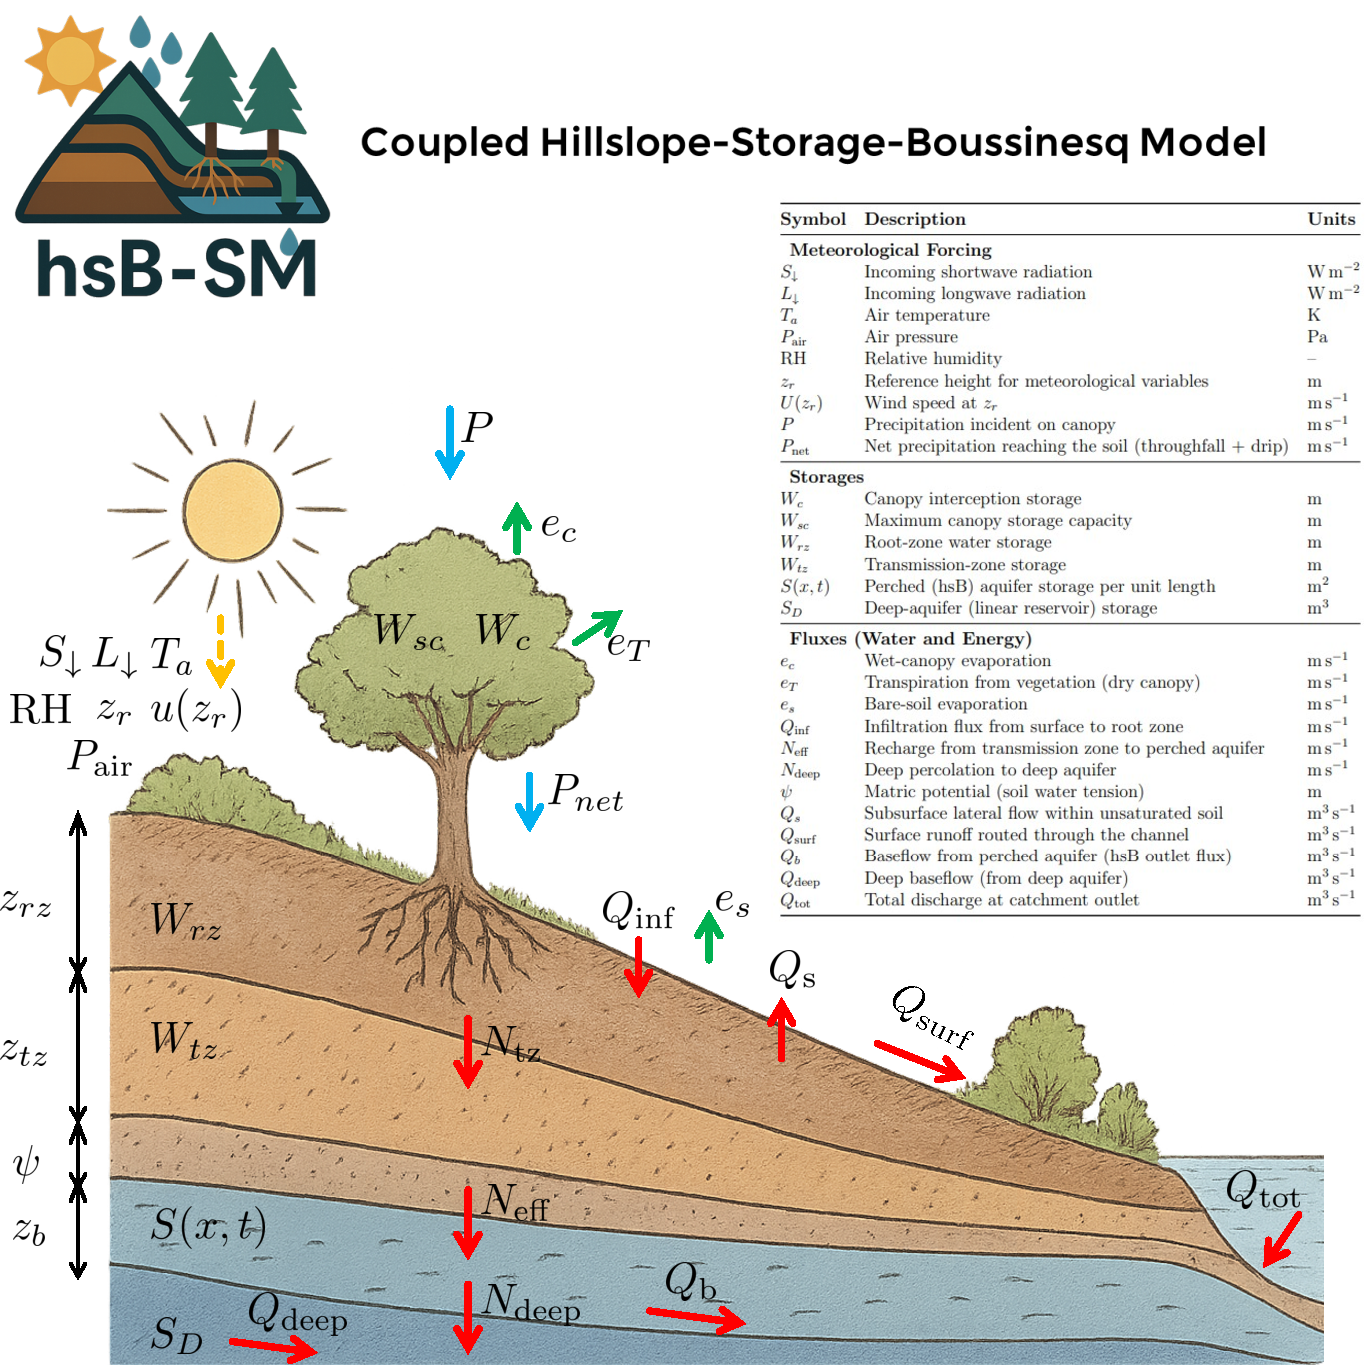
\includegraphics[width=1\linewidth]{Figures/hsB_Conceptual_Model.pdf}
    \caption{Five-store conceptual schematic inherited from the MATLAB manual. The active signed exchanges, soil saturation excess, and optional overflow redistribution are defined in Section~\ref{sec:rootzone}. The schematic does not show every implemented transfer.}
    \label{fig:placeholder}
\end{figure}

 \begin{table}[h!]
\centering
\caption{Summary of variables represented in the conceptual hsB--SM schematic.}
\begin{adjustbox}{max width=\linewidth}\begin{tabular}{@{}lll@{}}
\toprule
\textbf{Symbol} & \textbf{Description} & \textbf{Units} \\
\midrule
\multicolumn{3}{l}{\textbf{Meteorological Forcing}} \\
$S_\downarrow$ & Incoming shortwave radiation & W\,m$^{-2}$ \\
$L_\downarrow$ & Incoming longwave radiation & W\,m$^{-2}$ \\
$T_a$ & Air temperature & K \\
$P_{\mathrm{air}}$ & Air pressure & Pa \\
$e_a$ & Actual vapor pressure supplied as \texttt{VapP\_kPa} & kPa \\
$z_r$ & Reference height for meteorological variables & m \\
$U(z_r)$ & Wind speed at $z_r$ & m\,s$^{-1}$ \\
$P$ & Liquid water input (before canopy if interception is enabled) & m\,s$^{-1}$ \\
$P_{\text{net}}$ & Net precipitation reaching the soil (throughfall + drip) & m\,s$^{-1}$ \\
\midrule
\multicolumn{3}{l}{\textbf{Storages}} \\
$S_c$ & Canopy interception storage & m \\
$S_{sc}$ & Maximum canopy storage capacity & m \\
$S_{rz}$ & Root-zone water storage & m \\
$S_{tz}$ & Transmission-zone storage & m \\
$S(x,t)$ & Perched (hsB) aquifer storage per unit length & m$^{2}$ \\
$S_D$ & Deep-aquifer (linear reservoir) storage & m$^{3}$ \\
\midrule
\multicolumn{3}{l}{\textbf{Fluxes (Water and Energy)}} \\
$e_c$ & Wet-canopy evaporation & m\,s$^{-1}$ \\
$e_T$ & Transpiration from vegetation (dry canopy) & m\,s$^{-1}$ \\
$e_s$ & Bare-soil evaporation & m\,s$^{-1}$ \\
$Q_{\text{inf}}$ & Infiltration flux from surface to root zone & m\,s$^{-1}$ \\
$N_{\text{eff}}$ & Recharge from transmission zone to perched aquifer & m\,s$^{-1}$ \\
$N_{\text{deep}}$ & Deep percolation to deep aquifer & m\,s$^{-1}$ \\
$\psi$ & Matric potential (soil water tension) & m \\
$Q_{\text{surf}}$ & Surface runoff routed through the channel & m$^{3}$\,s$^{-1}$ \\
$Q_b$ & Baseflow from perched aquifer (hsB outlet flux) & m$^{3}$\,s$^{-1}$ \\
$Q_{\text{deep}}$ & Deep baseflow (from deep aquifer) & m$^{3}$\,s$^{-1}$ \\
$Q_{\text{tot}}$ & Total discharge at catchment outlet & m$^{3}$\,s$^{-1}$ \\
\bottomrule
\end{tabular}\end{adjustbox}
\end{table}

\section{Canopy Interception and Wet-Canopy Evaporation}
\label{sec:canopy}

\subsection{Conceptual Overview}

The canopy layer represents the interception and evaporation of precipitation on vegetation surfaces.
Precipitation incident on the vegetated fraction of the ground first fills a finite interception store on the canopy, which subsequently evaporates at a potential rate supplied by the Penman--Monteith (PM) formulation.
This component governs the partitioning of gross rainfall \(P\,[\mathrm{m\,s^{-1}}]\) into (i) intercepted water that evaporates, (ii) canopy drip, and (iii) direct throughfall reaching the soil surface.

The canopy process operates over the vegetated fraction \(f_v\in[0,1]\), while the open fraction \((1-f_v)\) transmits rainfall directly to the surface.
Within the vegetated fraction, a ``free throughfall'' coefficient \(f_0\in[0,1]\) allows a fraction of rainfall to bypass leaves and reach the ground without being stored in the canopy.

In what follows, all fluxes and storages are expressed \emph{per unit ground area}, so that the effects of the vegetation fraction are already embedded in the node-scale variables.
The node-scale wet-canopy evaporation \(E_{\mathrm{can}}\) is the same physical quantity as the wet-canopy component \(e_{wc}\) used in the energy-balance notation (Section~\ref{sec:energy_ET_partitioning}), simply expressed at the ground-area scale.

\subsection{Governing Water Balance}

The prognostic water balance for the canopy interception store, expressed per unit ground area \([\mathrm{m}]\), is
\begin{equation}
\frac{dS_{\mathrm{can}}}{dt}
  = P_{\mathrm{veg,eff}} - E_{\mathrm{can}} - D_{\mathrm{can}},
\label{eq:canopy_balance}
\end{equation}
where
\begin{itemize}
  \item \(S_{\mathrm{can}}\,[\mathrm{m}]\) is the intercepted water depth on the canopy (per unit ground area),
  \item \(E_{\mathrm{can}}\,[\mathrm{m\,s^{-1}}]\) is the actual node-scale evaporation rate from wet foliage, and
  \item \(D_{\mathrm{can}}\,[\mathrm{m\,s^{-1}}]\) is the drip (overflow) flux released from the canopy store to the ground.
\end{itemize}

Only the portion of rainfall that actually interacts with the canopy enters \(S_{\mathrm{can}}\).
The effective interception input (per ground area) is
\begin{equation}
P_{\mathrm{veg,eff}} = f_v (1 - f_0)\,P,
\label{eq:P_veg_eff}
\end{equation}
where
\begin{itemize}
  \item \(P\,[\mathrm{m\,s^{-1}}]\) is gross rainfall per ground area,
  \item \(f_v\) is the vegetated fraction, and
  \item \(f_0\) is the free-throughfall coefficient within the vegetated fraction.
\end{itemize}
Thus, \(f_v(1-f_0)P\) is the portion of rainfall that first fills the canopy store, while \(f_v f_0 P\) passes directly to the ground as free throughfall under the canopy.

\subsection{Storage Capacity and Effective Inputs}

The maximum interception capacity of the canopy is parameterized as a function of vegetation density and leaf area index (LAI):
\begin{equation}
W_{\mathrm{cap}} = f_v \, c_w \, \mathrm{LAI},
\label{eq:Wcap_def}
\end{equation}
where \(W_{\mathrm{cap}}\,[\mathrm{m}]\) is the maximum water depth that can be retained per unit ground area,
\(c_w\,[\mathrm{m\,LAI^{-1}}]\) is the canopy water capacity per unit LAI, and
LAI is the one-sided leaf area index.

The interception input \eqref{eq:P_veg_eff} and the capacity \eqref{eq:Wcap_def} together determine how quickly the canopy saturates during a storm and how much water is available for wet-canopy evaporation between storms.

\subsection{Evaporation from Wet Foliage}

Potential wet-canopy evaporation is supplied by the PM routine as a patch-scale rate \(e_{\mathrm{wetCan}}\,[\mathrm{m\,s^{-1}}]\) defined over the vegetated surface.
Converted to a node-scale (ground-area) potential flux, this becomes
\begin{equation}
E_{\mathrm{can}}^{\ast} = f_v\, e_{\mathrm{wetCan}}.
\label{eq:Ecan_potential}
\end{equation}

The actual wet-canopy evaporation rate is limited by water availability within the interception store.
Over a time step \(\Delta t\,[\mathrm{s}]\), the maximum amount that can evaporate is the sum of current storage and the interception input received during that step:
\begin{equation}
E_{\mathrm{can}} = \min\!\left(E_{\mathrm{can}}^{\ast},\;
\frac{S_{\mathrm{can}} + P_{\mathrm{veg,eff}}\,\Delta t}{\Delta t}\right).
\label{eq:Ecan_actual}
\end{equation}
This guarantees that evaporation cannot exceed either (i) the PM potential demand or (ii) the water that is actually present on the canopy.

\subsection{Overflow, Drip, and Updated Storage}

After applying interception input and evaporation, the provisional canopy store at the end of the step is
\begin{equation}
S_{\mathrm{can}}^{\star} = S_{\mathrm{can}} + P_{\mathrm{veg,eff}}\,\Delta t - E_{\mathrm{can}}\,\Delta t.
\label{eq:Scan_star}
\end{equation}
Any excess beyond the capacity \(W_{\mathrm{cap}}\) is released as overflow or drip,
\begin{equation}
D_{\mathrm{can}} =
\frac{\max\bigl(S_{\mathrm{can}}^{\star} - W_{\mathrm{cap}},\,0\bigr)}{\Delta t},
\label{eq:Dcan_def}
\end{equation}
All excess is released within the timestep. This matches the MATLAB canopy module at \texttt{Veg.drip\_coef=1}. Python does not expose a fractional drip coefficient: the legacy module discards the unreleased excess when that coefficient is below one and storage is clipped to capacity.

The remaining canopy storage at the end of the time step is then
\begin{equation}
S_{\mathrm{can}}^{(t+\Delta t)} =
S_{\mathrm{can}}^{\star} - D_{\mathrm{can}}\,\Delta t,
\label{eq:Scan_update}
\end{equation}
which ensures that \(0 \le S_{\mathrm{can}}^{(t+\Delta t)} \le W_{\mathrm{cap}}\).

\subsection{Throughfall and Ground-Reaching Precipitation}

The total ground-reaching rainfall rate, which becomes available for infiltration at the surface, combines:
\begin{enumerate}
  \item open-area rainfall over the non-vegetated fraction \((1-f_v)\),
  \item free throughfall within the vegetated fraction \(f_v f_0 P\), and
  \item canopy drip \(D_{\mathrm{can}}\) released from the interception store.
\end{enumerate}
At the node scale, the net precipitation to the ground is
\begin{equation}
P_{\mathrm{net}} = (1 - f_v)\,P \;+\; f_v f_0\,P \;+\; D_{\mathrm{can}}.
\label{eq:Pnet_canopy}
\end{equation}
By construction, \(P_{\mathrm{net}}\,[\mathrm{m\,s^{-1}}]\) is the quantity passed to the infiltration module at each computational node.
The wet-canopy evaporation \(E_{\mathrm{can}}\) contributes to the total evapotranspiration as the wet-canopy component.

\subsection{Conservation of Mass}

Using the definitions above, water is strictly conserved over the ground area.
Over a single time step \(\Delta t\), the node-scale water balance can be written as
\begin{equation}
P\,\Delta t = E_{\mathrm{can}}\,\Delta t
             + P_{\mathrm{net}}\,\Delta t
             + \bigl(S_{\mathrm{can}}^{(t+\Delta t)} - S_{\mathrm{can}}^{(t)}\bigr),
\label{eq:canopy_mass_conservation}
\end{equation}
which states that gross rainfall equals the sum of wet-canopy evaporation, net precipitation to the ground, and the change in canopy storage.
Substituting \eqref{eq:P_veg_eff}--\eqref{eq:Dcan_def} into \eqref{eq:canopy_balance} and \eqref{eq:Pnet_canopy} shows that \eqref{eq:canopy_mass_conservation} holds identically for any \(f_v\) and \(f_0\).

\subsection{Model Variables and Dimensions}

Table~\ref{tab:canopy_vars} maps equations to Python. Parameters belong to \texttt{config.params}; state and actual-flux outputs belong to \texttt{result.nodes}. Intermediate quantities are not automatically exported.

\begin{table}[H]
\centering
\caption{Primary variables used in the canopy interception module.}
\label{tab:canopy_vars}
\begin{adjustbox}{max width=\linewidth}\begin{tabular}{llll}
\toprule
Symbol & Description & Units & Code variable \\
\midrule
\(P\) & Gross rainfall rate (per ground area) & m\,s\(^{-1}\) & \texttt{forcing["P"]} \\
\(f_v\) & Vegetation cover fraction & -- & \texttt{forcing["fv"]} \\
LAI & Leaf area index (one-sided) & -- & \texttt{forcing["LAI"]} \\
\(f_0\) & Free-throughfall coefficient in vegetated fraction & -- & \texttt{Veg.free\_throughfall\_f0} \\
\(S_{\mathrm{can}}\) & Canopy water storage (per ground area) & m & \texttt{canopy\_m} \\
\(W_{\mathrm{cap}}\) & Maximum canopy storage capacity & m & \texttt{capacity (local)} \\
\(c_w\) & Storage capacity per unit LAI & m\,LAI\(^{-1}\) & \texttt{Veg.cw\_per\_LAI} \\
\(e_{\mathrm{wetCan}}\) & Potential wet-canopy evap (patch scale) & m\,s\(^{-1}\) & \texttt{pm["wet"] (local)} \\
\(E_{\mathrm{can}}^{\ast}\) & Potential canopy evap (ground scale) & m\,s\(^{-1}\) & \texttt{fv * pm["wet"] (local)} \\
\(E_{\mathrm{can}}\) & Actual canopy evaporation (ground scale) & m\,s\(^{-1}\) & \texttt{canopy\_evaporation\_mps} \\
\(D_{\mathrm{can}}\) & Canopy drip / overflow to ground & m\,s\(^{-1}\) & \texttt{drip / dt (local)} \\
\(P_{\mathrm{veg,eff}}\) & Effective interception input & m\,s\(^{-1}\) & \texttt{intercepted / dt (local)} \\
\(P_{\mathrm{net}}\) & Ground-reaching rainfall rate & m\,s\(^{-1}\) & \texttt{pnet (local)} \\
\bottomrule
\end{tabular}\end{adjustbox}
\end{table}

\subsection{Link to Potential Evapotranspiration Components}

In the time-stepping sequence, canopy interception is updated before infiltration and soil moisture.
Vegetation properties are drawn from \texttt{Params.Veg}, potential wet-canopy fluxes are obtained from the PM computation (Section~\ref{sec:potET_ra_rs}), and the canopy update is carried out by \texttt{physics.canopy\_step} (MATLAB: \texttt{hsbsm\_canopy\_pm}), which implements Eqs.~\eqref{eq:canopy_balance}--\eqref{eq:Pnet_canopy}.

The node-scale flux \(E_{\mathrm{can}}\) is then used as the wet-canopy evapotranspiration component in the energy-balance partitioning, while \(P_{\mathrm{net}}\) is passed to the infiltration and root-zone module.
When the canopy module is disabled, a pass-through fallback sets
\[
P_{\mathrm{net}} = P, \qquad E_{\mathrm{can}} = 0,
\]
This is the default in both active runners. Python uses \texttt{Flags.interception=false}. When input already represents liquid water reaching the soil, keep interception disabled; transpiration and soil evaporation remain active.




\section{Infiltration Capacity and Surface Partitioning}
\label{sec:infiltration}

\subsection{Conceptual Overview}
Infiltration converts ground-reaching precipitation into a vertical flux that enters the soil. The scheme computes a per-node infiltration capacity using Milly-type algebra and optionally limits conductivity with a moisture factor inspired by Troch-style controls. The incoming water at the surface, \(P_{\mathrm{net}}\,[\mathrm{m\,s^{-1}}]\), is partitioned at each node into an infiltrating flux \(I\,[\mathrm{m\,s^{-1}}]\), an infiltration-excess runoff \(R_{\mathrm{ex}}\,[\mathrm{m\,s^{-1}}]\) whenever supply exceeds capacity, and a saturation-excess term \(R_{\mathrm{sat}}\,[\mathrm{m\,s^{-1}}]\), which is kept zero in this module (saturation overland flow is handled elsewhere).

\subsection{Soil State, Effective Saturation, and Moisture Controls}
The model uses root-zone soil properties to represent near-surface hydraulic behavior. Volumetric water content at the node, \(\theta[-]\), is either passed from the state or defaults to \(\theta_0\). Effective saturation is
\[
S_e=\frac{\theta-\theta_r}{\theta_s-\theta_r}, \qquad S_e\in [S_{e,\min},\,1],
\]
where \(\theta_s\) is porosity, \(\theta_r\) is the residual water content, and \(S_{e,\min}\) is a small floor to avoid degeneracy. When the optional Troch control is active, a moisture factor \(c=\min(S_e,\,c_{\max})\) limits the effective hydraulic conductivity used in the capacity calculation. In the default Milly mode, conductivity is not reduced by \(c\).

\subsection{Sorptivity and Effective Conductivity}
The capacity expression combines two physical controls: an effective conductivity \(K_{\mathrm{eff}}\) and a sorptivity \(S\,[\mathrm{m\,s^{-1/2}}]\) that represents the capillary drive of an advancing wetting front. Users may override \(S\) directly; in that case the code skips the internal estimate. Otherwise, \(S\) is estimated from soil parameters using a Milly-style proxy,
\[
S \;\approx\; \sqrt{\frac{2\,\Delta\theta\,K_{\mathrm{base}}}{\alpha_{\mathrm{eff}}}},
\qquad \Delta\theta=\max(\theta_s-\theta,\,0),
\]
where \(K_{\mathrm{base}}\,[\mathrm{m\,s^{-1}}]\) is the root-zone saturated hydraulic conductivity and \(\alpha_{\mathrm{eff}}\,[\mathrm{m^{-1}}]\) is taken from van Genuchten $\alpha$, unless \texttt{Infil.model="Troch"} and a positive \texttt{Troch.alpha\_inv\_m} is supplied. Despite its inherited name, this override is a capillary length in m; $\alpha_{\mathrm{eff}}=1/\texttt{Troch.alpha\_inv\_m}$. It has no effect in Milly mode or when sorptivity is supplied directly. The effective conductivity is
\[
K_{\mathrm{eff}}=
\begin{cases}
c\,K_{\mathrm{base}}, & \text{Troch mode (moisture-limited)},\\
K_{\mathrm{base}}, & \text{Milly mode}.
\end{cases}
\]

\subsection{Milly Capacity and Supply--Capacity Partitioning}
Let \(F\,[\mathrm{m}]\) be the cumulative infiltrated depth at the beginning of the time step. The Milly algebra used in the code produces a closed-form infiltration \emph{capacity} \(I_{\max}\,[\mathrm{m\,s^{-1}}]\),
\[
I_{\max}=K_{\mathrm{eff}}+\frac{S^2}{2\max(F,F_{\min})},
\]
where $F_{\min}>0$ is the cumulative-depth floor (default 0.01 m). This expression transitions from sorptivity control (early times, small \(F\)) to conductivity control (late times, large \(F\)). The actual infiltration rate is the minimum between the water supply and the capacity,
\[
I \;=\; \min\!\bigl(P_{\mathrm{net}},\, I_{\max}\bigr).
\]
Infiltration-excess runoff forms when supply exceeds capacity:
\[
R_{\mathrm{ex}} \;=\; \max\!\bigl(P_{\mathrm{net}}-I,\,0\bigr).
\]
Saturation-excess runoff is not generated by this module, i.e., \(R_{\mathrm{sat}}=0\); any perched or saturation-driven overland flow is computed in the corresponding saturation component of the model.

\subsection{Cumulative Infiltration Update and Dry-Step Reset}
The cumulative infiltrated depth is advanced as
\[
F^{(t+\Delta t)} \;=\; F^{(t)} + I\,\Delta t,
\]
with \(\Delta t\,[\mathrm{s}]\) the model time step. A dry-step counter is incremented when \(P_{\mathrm{net}}=0\). The reset occurs when the counter exceeds \texttt{Infil.resetDrySteps}, and sets $F=\max(F_0,F_{\min})$ and the counter to zero. With the defaults of three dry steps, $F_0=0.001$ m and $F_{\min}=0.01$ m, the fourth consecutive dry step resets $F$ to 0.01 m. Initial cumulative depth is separately set by \texttt{initial.infiltration\_m} (default zero).

\subsection{Mass Balance at the Surface}
At each node and time step, the surface water budget is
\[
P_{\mathrm{net}}\,\Delta t \;=\; I\,\Delta t \;+\; R_{\mathrm{ex}}\,\Delta t \;+\; R_{\mathrm{sat}}\,\Delta t,
\]
with \(R_{\mathrm{sat}}=0\) inside this module. The infiltrated volume joins the soil water balance of the root zone in the next subcomponent.

\subsection{Variables, Parameters, and Code Correspondence}
Table~\ref{tab:infiltration_vars} lists Python quantities. Among the local infiltration variables below, only \texttt{infiltration\_mps} and layer states are exported. Total runoff is exported as \texttt{surface\_runoff\_mps}.

\begin{table}[H]
\centering
\caption{Primary variables and parameters for infiltration capacity and partitioning.}
\label{tab:infiltration_vars}
\begin{adjustbox}{max width=\linewidth}\begin{tabular}{llll}
\toprule
Symbol & Description & Units & Code variable \\
\midrule
\(P_{\mathrm{net}}\) & Ground-reaching rainfall supply & m\,s\(^{-1}\) & \texttt{pnet (local)} \\
\(I\) & Actual infiltration rate & m\,s\(^{-1}\) & \texttt{infiltration\_mps} \\
\(R_{\mathrm{ex}}\) & Infiltration-excess runoff rate & m\,s\(^{-1}\) & \texttt{rex (local)} \\
\(R_{\mathrm{sat}}\) & Saturation-excess runoff rate & m\,s\(^{-1}\) & \texttt{zero in infiltration} (=0 here) \\
\(F\) & Cumulative infiltrated depth & m & \texttt{cumulative (local)} \\
\(\theta\) & Volumetric water content & -- & \texttt{theta} (from \texttt{theta\_rz}) \\
\(\theta_s,\theta_r\) & Saturated and residual water contents & -- & \texttt{Soil.RZ.theta\_sat/theta\_min} \\
\(S_e\) & Effective saturation & -- & derived from \(\theta\) \\
\(S\) & Sorptivity (capillary drive) & m\,s\(^{-1/2}\) & \texttt{sqrt(s2) (local)} (diagnostic) \\
\(K_{\mathrm{base}}\) & Base saturated conductivity (RZ) & m\,s\(^{-1}\) & \texttt{Soil.RZ.vG.Ks} or \texttt{Infil.K\_mps} \\
\(K_{\mathrm{eff}}\) & Effective conductivity (after moisture limit) & m\,s\(^{-1}\) & internal \\
\(\alpha\) & van Genuchten inverse capillary length & m\(^{-1}\) & \texttt{Soil.RZ.vG.alpha} \\
\(\alpha_{\mathrm{eff}}\) & Effective inverse capillary length & m\(^{-1}\) & \texttt{Troch.alpha\_inv\_m}\({}^{-1}\) or \(\alpha\) \\
\(c\) & Moisture factor (Troch) & -- & from \(S_e\), capped by \texttt{Infil.max\_c} \\
\(S_{\mathrm{user}}\) & User-provided sorptivity override & m\,s\(^{-1/2}\) & \texttt{Infil.S\_mps05} \\
\(\Delta t\) & Time step & s & \texttt{dt} \\
\bottomrule
\end{tabular}\end{adjustbox}
\end{table}

% \subsection{Implementation Notes}
% The runner calls a safe wrapper that attempts the user-selected infiltration function and falls back to a minimal partitioner if needed:
% \[
% [\mathbf{I},\mathbf{R}_{\mathrm{ex}},\mathbf{R}_{\mathrm{sat}},S_{\mathrm{Inf}}]
% =\texttt{local\_safe\_infiltration\_vec}(\texttt{Fns.infiltration},\mathbf{P}_{\mathrm{net}},S_{\mathrm{Inf}},\texttt{Params},\Delta t,\boldsymbol{\theta},N_x).
% \]
% The Milly/Troch function adheres to the signature \texttt{Fns.infiltration(pnet (local),SInf,Params,dt,theta)} and must return node-length column vectors for \(I\), \(R_{\mathrm{ex}}\), \(R_{\mathrm{sat}}\) (zero in this module), and an updated \texttt{SInf} with the cumulative infiltration \(F\). The state also keeps a dry-step counter that triggers resetting \(F\) to \(F_0\) after a configurable number of consecutive dry steps, with thresholds that may depend on \(\Delta t\).


% ============================================================
% hsB-SM Technical Manual
% Part 2 -- Root Zone and Transmission Zone Balances
% ============================================================
\section{Coupled Root-Zone, Transmission-Zone, and Aquifer Exchange}
\label{sec:rootzone}
\label{subsec:tz_dynamics}

The active MATLAB runner uses \texttt{hsbsm\_rz\_tz\_coupled}. The Python function \texttt{hsbsm.physics.soil\_step} uses the same hydraulic closures and signed Darcy gradients. This section replaces the duplicated independent root-zone descriptions in the original manual. It distinguishes the transfer equations from the conservative limits applied during each timestep.

\subsection{States and hydraulic properties}

For each layer $j\in\{r,t\}$, let $z_j$ [m] be its thickness and $\theta_j$ [m$^3$\,m$^{-3}$] its water content. Its storage depth is $W_j=z_j\theta_j$ [m]. Residual and saturated bounds are $W_{j,\min}=z_j\theta_{j,\min}$ and $W_{j,\max}=z_j\theta_{j,s}$. The effective saturation and van Genuchten--Mualem closures are
\begin{align}
S_{e,j}&=\frac{\theta_j-\theta_{j,\min}}{\theta_{j,s}-\theta_{j,\min}},\qquad m_j=1-\frac{1}{n_j},\\
\psi_j&=-\frac{(S_{e,j}^{-1/m_j}-1)^{1/n_j}}{\alpha_j},\\
K_j&=K_{s,j}S_{e,j}^{1/2}\left[1-(1-S_{e,j}^{1/m_j})^{m_j}\right]^2.
\end{align}
Here $\psi_j$ [m] is pressure head, $K_j$ [m\,s$^{-1}$] is unsaturated conductivity, $\alpha_j$ [m$^{-1}$] and $n_j>1$ are retention parameters, and $K_{s,j}$ is saturated conductivity. The code regularizes effective saturation near zero and caps pressure head at $-10$ m in RZ and $-20$ m in TZ, matching the source module.

\subsection{Potential demand, stress, and available water}
\label{subsec:rz_stress}
\label{subsec:sl_stress}

The PM module supplies transpiration potential $T^*$ and soil evaporation potential $E_s^*$ over ground area. The active coupling applies the source's linear pressure-head factors
\begin{equation}
f_T=\operatorname{clip}\left(\frac{\psi_r+10}{9},0,1\right),\qquad
f_E=\operatorname{clip}\left(\frac{\psi_r+10}{9.5},0,1\right).
\end{equation}
Let $A_r=\max(W_r-W_{r,\min},0)$ [m] be the initially removable root-zone water. Actual transpiration and soil evaporation are
\begin{align}
T&=\min(f_T T^*,A_r/\Delta t),\label{eq:etrz_limit}\\
E_s&=\min\left(f_E E_s^*,\max(A_r/\Delta t-T,0)\right).\label{eq:esoil_limit}
\end{align}
Both rates have units m\,s$^{-1}$. Sharing the donor water prevents both fluxes from independently spending the same storage. Infiltration $I$ is then included in the provisional root-zone store, $W_r^*=W_r+(I-T-E_s)\Delta t$.

\subsection{Signed exchange between RZ and TZ}

With elevation positive upward and the ground surface at zero, the layer centers are $Z_r=-z_r/2$ and $Z_t=-(z_r+z_t/2)$. The unconstrained downward-positive exchange is
\begin{equation}
q_{rt}=\frac{K_r+K_t}{2}\,
\frac{(\psi_r+Z_r)-(\psi_t+Z_t)}{(z_r+z_t)/2}.
\end{equation}
Negative $q_{rt}$ represents capillary return to the root zone. The flux is limited by removable donor water in the corresponding direction, then debited from one store and credited to the other. The arithmetic-mean conductivity follows the active source module. No second capillary-demand bookkeeping step is applied.

\subsection{TZ--aquifer interface and recharge split}

The inherited coupling interprets aquifer head $h_a\ge0$ as water-table height relative to the bottom of the transmission zone for evaluating the interface gradient. This is a conceptual coupling convention; the soil buckets and the lateral hsB storage remain separate prognostic stores. Define $d_w=\min(h_a,z_t)$ and $L_u=\max(z_t-d_w,10^{-3})$ [m]. The unconstrained interface flux is
\begin{equation}
q_{ta}=K_t\frac{\psi_t+z_t/2-d_w}{L_u}.
\end{equation}
Positive flux is downward drainage and negative flux is aquifer-to-TZ return. The negative branch is multiplied by \texttt{Soil.TZ.cap\_frac\_of\_K}, with default 0.30. Downward transfer is limited by remaining TZ donor water; upward transfer is limited by aquifer water depth $S/w=fh_a$ and the receiving TZ capacity.

Only the downward part is divided between perched and deep recharge. With $q^+=\max(q_{ta},0)$ and $q^-=\max(-q_{ta},0)$,
\begin{equation}
N_{\mathrm{hsB}}=(1-\phi_d)q^+-q^-,\qquad
N_{\mathrm{deep}}=\phi_d q^+.
\label{eq:split_recharge}
\end{equation}
The parameter $\phi_d\in[0,1]$ is \texttt{Deep.phi\_d}. Negative net perched recharge is withdrawn before lateral integration. The deep reservoir receives only downward transfer and releases water according to the available-water-limited linear reservoir update.

\subsection{Storage closure and saturation excess}

After the signed transfers, any storage above a layer's saturated capacity is recorded as surface runoff $R_r$ or $R_t$ [m\,s$^{-1}$]. It is never discarded by clipping. The layer balances are
\begin{align}
\Delta W_r&=(I-T-E_s-q_{rt}-R_r)\Delta t,\\
\Delta W_t&=(q_{rt}-q_{ta}-R_t)\Delta t.\label{eq:tz_balance}
\end{align}
The internal exchange $q_{rt}$ cancels when the balances are added. Python exports signed exchange rates, both layer states, actual ET, and surface runoff for auditing. This treatment changes source cases in which the old module clipped storage after incompatible flux demands.

\newpage


\section{Surface Runoff Generation and Baseflow/Channel Routing}
\label{sec:surface_runoff}

This section specifies how hsB-SM converts precipitation into (i) \emph{surface runoff} that is \emph{routed through the channel network} using a linearized de Saint--Venant response, and (ii) \emph{subsurface baseflow} generated by the hillslope-storage Boussinesq (hsB) aquifer, which is \emph{delivered instantaneously at the outlet}. We also account for a \emph{deep aquifer} partition of percolation (transmission-zone drainage), which may act as a slow baseflow reservoir.

\subsection{Runoff production at the land surface}

At each node, infiltration is $I=\min(P_{\mathrm{net}},f_{\mathrm{cap}})$. The infiltration module returns
\begin{equation}
r_{\mathrm{ex}}=P_{\mathrm{net}}-I,\qquad r_{\mathrm{sat,infil}}=0.
\label{eq:rex}
\end{equation}
Soil excess $R_r+R_t$ is computed after the coupled soil transfers. Let $Q_{\mathrm{of},j}$ [m$^3$\,s$^{-1}$] be aquifer overflow remaining after any optional redistribution into TZ and RZ. Then
\begin{equation}
r_{\mathrm{sat},j}=R_{r,j}+R_{t,j}+Q_{\mathrm{of},j}/A_j,
\label{eq:rsat}
\end{equation}
\begin{equation}
r_{\mathrm{node},j}=r_{\mathrm{ex},j}+r_{\mathrm{sat},j}.
\label{eq:r-total}
\end{equation}
These rates are already expressed per unit ground area. No further vegetation weighting is applied. Defining a second runoff term as $P_{\mathrm{net}}-I$ would count infiltration excess twice. Python also corrects the legacy runner's second addition of aquifer overflow at the outlet.

For hsB cell $j$ with planform area $A_j$ [m$^2$], the lateral inflow to the channel network (discharge units) is
\begin{equation}
R_j(t) \;=\; r_{\text{node},j}(t)\, A_j \qquad [\mathrm{m^3\,s^{-1}}],
\label{eq:Rj}
\end{equation}
and the reach-aggregated lateral inflow series is
\begin{equation}
R_L(t) \;=\; \sum_{j=1}^{N_x} R_j(t).
\label{eq:RL}
\end{equation}
Hence, the propagation time from the hillslope to the nearest channel is neglected.

\subsection{Transmission-zone drainage: partition to perched hsB and deep aquifer}

Let $g_{tz}=\max(q_{ta},0)$ denote downward TZ drainage and $q^-=\max(-q_{ta},0)$ denote upward return. Only downward drainage is split:
\begin{equation}
N_{\text{hsB}}(x,t) \;=\; \bigl(1-\phi_d\bigr)\, g_{tz}(x,t)-q^-(x,t),
\qquad
N_{\text{deep}}(x,t) \;=\; \phi_d\, g_{tz}(x,t),
\label{eq:split}
\end{equation}
where $\phi_d\in[0,1]$ is the deep-aquifer fraction (user-specified or calibrated).

The field $N_{\text{hsB}}(x,t)$ is the vertical recharge boundary that drives lateral subsurface flow in the hsB solver. Deep recharge remains in the modeled deep store until released to the outlet. Its continuous linear-reservoir balance is
\begin{equation}
\frac{dS_D}{dt} \;=\; \int_0^{L} N_{\text{deep}}(x,t)\, w(x)\, dx \;-\; Q_D(t),
\qquad
Q_D(t) \;=\; k_D\, S_D(t),
\label{eq:deep}
\end{equation}
where $S_D$ is deep storage, $Q_D$ the deep baseflow discharge at the outlet, $w(x)$ the planform width, and $k_D>0$ a reservoir coefficient. Setting $k_D=0$ retains water in the deep store without return flow during the run; it remains part of the water balance. The actual discrete update first adds recharge, then releases $\min[k_D(S_D+N_D\Delta t), (S_D+N_D\Delta t)/\Delta t]$, using consistent volume units. This matches the input-first MATLAB reservoir update. Alternatively, $k_D$ can be estimated with recession analysis. One can define the master recession curve and partition the flow discharges into rapid-perched, Boussinesq aquifer, and low-deep aquifer flows. By fitting a power-law relationship for the slow part of the recession, one can estimate $k_D$, especially if a linear reservoir is assumed.

\subsection{Hillslope baseflow from hsB (instantaneous at the outlet)}

Given the perched-aquifer recharge field $N_{\text{hsB}}(x,t)$ from Part~2, the hsB module computes lateral groundwater flow along a 1D hillslope using a conservative finite-volume formulation of the storage--Boussinesq equations (see the accompanying hsB manual). The prognostic state is the storage per unit-$x$,
\begin{equation}
S(x,t) \;=\; f\,w(x)\,h(x,t), \qquad h(x,t)\ge 0,
\label{eq:hsb-state}
\end{equation}
with constant drainable porosity $f$ and coordinate $x$ increasing from outlet to divide, planform width $w(x)>0$, and water-table height $h$ above bedrock. Over each cell $[x_{i-\frac12},x_{i+\frac12}]$, conservation reads
\begin{equation}
\frac{\mathrm d}{\mathrm dt}\int_{x_{i-\frac12}}^{x_{i+\frac12}} S\,\mathrm dx
\;=\;
Q\!\left(x_{i-\frac12},t\right) \;-\; Q\!\left(x_{i+\frac12},t\right)
\;+\; \int_{x_{i-\frac12}}^{x_{i+\frac12}} N_{\text{hsB}}(x,t)\,w(x)\,\mathrm dx,
\label{eq:hsb-fv}
\end{equation}
where the Dupuit--Boussinesq discharge along $x$ is split into a diffusive gradient term and a downslope drift term,
\begin{equation}
Q(x,t) \;=\; -\frac{k}{f}
\left[
S(x,t)\,\cos\iota\,\frac{\partial h}{\partial x}(x,t)
\;+\; S(x,t)\,\sin\iota
\right].
\label{eq:hsb-flux}
\end{equation}

\paragraph{Finite volumes and face fluxes.}
We store $S_i(t)\approx S(x_i,t)$ at cell centers. Face fluxes $Q_{i+\frac12}$ are assembled with a robust split:
\begin{align}
Q_{i+\frac12}
&= Q^{\text{diff}}_{i+\frac12} + Q^{\text{adv}}_{i+\frac12} + Q^{\text{num}}_{i+\frac12}, \\
Q^{\text{diff}}_{i+\frac12}
&= -\frac{k\cos\iota}{f}\;S^{H}_{i+\frac12}\;\frac{h_{i+1}-h_i}{x_{i+1}-x_i},\qquad
S^{H}_{i+\frac12}=\frac{2\,\widehat S_i\,\widehat S_{i+1}}{\widehat S_i+\widehat S_{i+1}},\\
Q^{\text{adv}}_{i+\frac12}
&= -\frac{k\sin\iota}{f}\;S^{\text{up}}_{i+\frac12},\qquad
S^{\text{up}}_{i+\frac12}=\begin{cases} S_i, & \text{downslope flow},\\ S_{i+1}, & \text{upslope (rare)},\end{cases}\\
Q^{\text{num}}_{i+\frac12}
&= \tfrac12\,a\,(S_i-S_{i+1}),\qquad a=2\left|\frac{k\sin\iota}{f}\right|.
\end{align}
A small head floor inside $\widehat S$ keeps $S^{H}$ strictly positive near the seepage face, improving robustness.

\paragraph{Time integration and nonlinear iteration.}
The semi-discrete system is advanced by a $\theta$-method (default $\theta=1$, backward Euler):
\begin{equation}
\frac{S^{n+1}_i-S^n_i}{\Delta t}
\;=\;
-\frac{Q_{i+\frac12}(S^{n+\theta})-Q_{i-\frac12}(S^{n+\theta})}{\Delta x_i}
\;+\; \bigl[N_{\text{hsB}}\,w\bigr]^n_i,
\label{eq:hsb-theta}
\end{equation}
with Picard linearization and relaxation to resolve the nonlinearity $h=S/(f\,w)$ inside $Q(\cdot)$. In the native-forcing mode, internal substeps $\Delta t_{\text{sub}}$ are chosen adaptively via advective and diffusive CFL-like limits then exactly tile each forcing interval. Python also checks convergence and retries failed substeps; the forcing-interval mean discharge and final state are reported for each row.

\paragraph{Boundary conditions and sign convention.}
A seepage boundary at the outlet imposes $h(0,t)=0$ (Dirichlet head), closed by a one-sided gradient for $Q^{\text{diff}}$; the divide enforces $Q(L,t)=0$. Internally, outward subsurface flow at the outlet face $x=0$ (indexed by $1/2$) is negative: $Q_{\frac12}(t)<0$.

\paragraph{Finite thickness and saturation-excess.}
If a finite aquifer thickness $D$ is specified, the solver clips $h\le D$ each substep and converts any storage overflow to an outlet-equivalent saturation-excess discharge $Q_{\text{surf,hsB}}$ to preserve mass. In Python, overflow enters the surface-routing inflow once. If fill-spill is enabled, it first fills remaining TZ and RZ capacity at the originating node, and the remainder enters routing.

\paragraph{Mass-balance diagnostics.}
At every accepted step, the code reports a domain-integrated residual in volume units, computed from the accepted flux divergence, recharge source, and any overflow sink; this residual should remain near machine/iteration tolerances.

\paragraph{Outlet baseflow.}
The instantaneous \emph{baseflow} contributed by the perched aquifer is the outward-positive outlet flux
\begin{equation}
Q_{\text{base}}(t) \;=\; -\,Q_{\frac12}(t),
\label{eq:hsb-qbase}
\end{equation}
which is added directly by default. Python can optionally route baseflow through the same channel kernel. In post-processing, $Q_{\text{base}}$ can be converted to an areal rate (e.g., mm\,day$^{-1}$) by dividing by the hillslope plan area $A_{\text{hs}}=\sum_i w_i\Delta x_i$ and multiplying by $1000\times 86400$.


\subsection{Channel routing of surface runoff (linearized de Saint--Venant)}

Surface runoff produced on the hillslope is routed through the channel network using the analytic impulse response of the \emph{linearized de Saint--Venant} model. The (drift--diffusion) impulse response at downstream distance $x$ is
\begin{equation}
q_c(x,t) \;=\; \frac{x}{\sqrt{2\pi}\, d\, t^{3/2}}\;
\exp\!\left[-\,\frac{\bigl(x - c\, t\bigr)^2}{2\, d^2\, t}\right],
\label{eq:qcx}
\end{equation}
where $c$ [m\,s$^{-1}$] is celerity and $d^2$ [m$^2$\,s$^{-1}$] is the dispersion parameter. Both implementations derive these from velocity $V$, Froude number $F$, coefficient $a_0$, and channel slope $S_0$:
\begin{equation}
c=(1+a_0)V,\qquad d^2=\frac{V^3}{gS_0F^2}(1-a_0^2F^2),
\end{equation}
with $g=9.80665$ m\,s$^{-2}$. Python requires $S_0,V,F>0$ and $0\le a_0F<1$.

Let $W_c(x)$ be the normalized channel width function (probability density over flow distances to the outlet). The \emph{network unit hydrograph} is obtained by geomorphic averaging:
\begin{equation}
u_c(t) \;=\; \int_{0}^{\infty} q_c(x,t)\, W_c(x)\, dx,
\label{eq:uc}
\end{equation}
which satisfies $\int_0^\infty u_c(t)\,dt = 1$. The routed surface-flow discharge at the outlet is the convolution of lateral inflows with $u_c$:
\begin{equation}
Q_{\text{surf}}(t) \;=\; \int_{0}^{t} R_L(\tau)\, u_c\!\bigl(t-\tau\bigr)\, d\tau.
\label{eq:Qsurf}
\end{equation}
In practice, $u_c(t)$ is precomputed from \eqref{eq:qcx}--\eqref{eq:uc} given $(c,d^2)$ and $W_c$, and \eqref{eq:Qsurf} is evaluated efficiently by FFT-based convolution on the model time step.


\subsection{Total outlet discharge and bookkeeping}

The total outward-positive discharge at the outlet is the sum of routed surface flow, instantaneous hsB baseflow, and (optionally) deep-reservoir outflow:
\begin{equation}
Q_{\text{tot}}(t) \;=\; Q_{\text{surf}}(t) \;+\; Q_{\text{base}}(t) \;+\; Q_D(t).
\label{eq:Qtot}
\end{equation}
Mass conservation is enforced by consistent use of units and areas: node runoff depths $r_{\text{node}}$ are converted to discharges via \eqref{eq:Rj}, transmission-zone drainage is split by \eqref{eq:split}, and hsB receives $N_{\text{hsB}}$ as its recharge field. The deep component remains in storage or returns through the linear reservoir in Eq.~\eqref{eq:deep}. Upward aquifer-to-TZ transfer is subtracted from net perched recharge as in Eq.~\eqref{eq:split_recharge}.

\subsection{Implementation notes}

\begin{itemize}
  \item \textbf{Units.} Work internally with m\,s$^{-1}$ for fluxes and m$^3$\,s$^{-1}$ for discharges. For plotting, convert to mm\,day$^{-1}$ by dividing discharges by $A_{\text{hs}}$ and multiplying by $1000\times 86400$.
  \item \textbf{Sequence per time step.} (i) compute $r_{\text{node},j}$ and $R_j$; (ii) form $R_L$; (iii) compute $N_{\text{hsB}}$ and advance hsB to get $Q_{\text{base}}$; (iv) convolve $R_L$ with $f_c$ to obtain $Q_{\text{surf}}$; (v) advance deep reservoir \eqref{eq:deep}; (vi) assemble $Q_{\text{tot}}$ via \eqref{eq:Qtot}.
  \item \textbf{Parameters.} Configure \texttt{Route.V}, \texttt{Route.F}, \texttt{Route.a0}, channel slope, and channel-distance weights. Both normal parameter-building paths derive $(c,d^2)$ from these quantities. Python does not accept direct \texttt{Route.c}, \texttt{Route.d}, or \texttt{Route.d2} overrides. The deep branch uses $(\phi_d,k_D)$.
  \item \textbf{Special case (finite aquifer thickness).} Overflow due to finite $D$ is included once in surface inflow before channel routing. The diagnostic overflow series must not be added again to the final outlet discharge.
\end{itemize}

% ============================================================
% hsB--SM Technical Manual
% Energy Balance and Evapotranspiration Partitioning
% (explicit soil-moisture stress functions, FW94 notation)
% ============================================================

\section{Energy Balance and Evapotranspiration Partitioning}
\label{sec:energy_ET_partitioning}

Penman--Monteith supplies three patch-scale potential rates, wet-canopy evaporation, dry-canopy transpiration, and bare-soil evaporation. They are converted to ground-area demand by multiplying the canopy components by $f_v$ and the bare-soil component by $1-f_v$. The optional snow-cover fraction further multiplies bare-soil demand by $1-\mathrm{SFC}$. These potential rates enter the storage updates described in Sections~\ref{sec:canopy} and \ref{sec:rootzone}.

The wet-canopy actual rate is limited by intercepted water, including the within-step rain input. Root-zone transpiration and soil evaporation use the pressure-head stress factors and the shared donor-water limits in Eqs.~\eqref{eq:etrz_limit}--\eqref{eq:esoil_limit}. The active coupling therefore includes stress factors as well as availability limits. The older independent-bucket availability-only formulation is not the Python default.

The node-scale actual evapotranspiration rate is
\begin{equation}
E=E_{\mathrm{can}}+T+E_s.
\label{eq:et_sum_actual}
\end{equation}
All terms are water depth rates in m\,s$^{-1}$ over ground area. Canopy evaporation is debited from the canopy store; transpiration and soil evaporation are debited from RZ. Internal hydraulic exchanges redistribute water and do not contribute to atmospheric loss. The model calculates potential rates using PM but does not independently solve surface temperature or close the sensible-heat energy balance.

\section{Computation of Potential Evapotranspiration and Aerodynamic Resistances}
\label{sec:potET_ra_rs}

The following equations describe the active MATLAB and Python PM calculation. All three potential components share net radiation and aerodynamic resistance. Separate surface temperatures, stability corrections, Jarvis modifiers, and stage-2 exfiltration are not configurable parts of this implementation.

\subsection{Meteorological quantities}
Temperature is supplied as $T_C$ [$^\circ$C], pressure and actual vapor pressure as $p$ and $e_a$ [kPa]. Set $T_K=T_C+273.15$. The active approximations are
\begin{align}
e_s&=0.6108\exp\left(\frac{17.27T_C}{T_C+237.3}\right),\\
\Delta&=\frac{4098e_s}{(T_C+237.3)^2},\qquad \mathrm{VPD}=\max(e_s-\max(e_a,0),0),\\
\rho_a&=\frac{1000p}{287T_K},\qquad \gamma=\frac{1005p}{0.622(2.45\times10^6)}.
\end{align}
Here $\Delta$ and $\gamma$ have units kPa\,K$^{-1}$ and $\rho_a$ has units kg\,m$^{-3}$. Actual vapor pressure is an input; relative humidity is not a required column.

\subsection{Radiation and aerodynamic resistance}
The shared net radiation is
\begin{equation}
R_n=(1-\operatorname{clip}(\mathrm{Albd},0,0.95))\max(S_\downarrow,0)
+0.98\left(L_\downarrow-\sigma T_K^4\right),
\end{equation}
with $\sigma=5.670374419\times10^{-8}$ W\,m$^{-2}$\,K$^{-4}$ and ground heat flux $G=0$.
Use $d=0.65h_c$, $z_{0m}=\max(0.001,0.10h_c)$ and $z_{0h}=\max(0.0001,0.10z_{0m})$, all in m, unless the corresponding \texttt{Veg} parameter is supplied. If the reference height $z_r\le d$, the calculation uses $z_r=d+z_{0m}+1$ m. The common resistance is
\begin{equation}
r_a=\max\left[5,\frac{\ln((z_r-d)/z_{0m})\ln((z_r-d)/z_{0h})}
{0.41^2\max(U,0.1)}\right].
\label{eq:ra_neutral}
\end{equation}
Wind speed is in m\,s$^{-1}$ and $r_a$ in s\,m$^{-1}$. Supplied measurement and vegetation heights should be physically consistent even though this numerical fallback is available.

\subsection{Three potential rates and actual ET}
For a surface resistance $r_s$ [s\,m$^{-1}$], the potential water-depth rate is
\begin{equation}
e^*(r_s)=\max\left[0,\frac{1000\Delta R_n+\rho_a1005(1000\mathrm{VPD})/r_a}
{2.45\times10^9\left[1000\Delta+1000\gamma(1+r_s/r_a)\right]}\right].
\label{eq:PM_wc}
\end{equation}
The wet-canopy rate uses $r_s=0$; dry-canopy transpiration uses $r_s=r_{c,\min}/\max(\mathrm{LAI},0.1)$; bare-soil evaporation uses \texttt{Soil.rs\_soil} (default 157.70 s\,m$^{-1}$). The factors of 1000 convert kPa to Pa. The latent-heat and water-density product is $2.45\times10^9$ J\,m$^{-3}$, giving rates in m\,s$^{-1}$.

Canopy demands are multiplied by $f_v$ and bare-soil demand by $(1-f_v)(1-\mathrm{SFC})$. Missing snow-cover fraction defaults to zero. The canopy and coupled soil updates then impose water availability and pressure-head stress. Actual rates are added once in Eq.~\eqref{eq:et_sum_actual}; there is no second vegetation weighting or separate stage-2 capacity.

%

% Reference Tables -- Variables and Parameters
% ============================================================
\section{Python Interfaces, Numerical Checks, and Reproducibility}
\label{sec:python_reference}

\subsection{Configuration and array conventions}

\texttt{load\_config(path)} returns a \texttt{Config} object containing \texttt{grid}, \texttt{forcing}, \texttt{dt}, \texttt{channel}, \texttt{params}, \texttt{initial}, and \texttt{metadata}. Geometry arrays contain one value per cell. Node outputs have shape $(N_t,N_x)$, with time on the first axis. A timestamp marks the beginning of a forcing interval; the reported storage at that row is the state after advancing that interval. Discharge and flux entries are interval-mean rates.

The input forcing is spatially uniform. It contains \texttt{date}, precipitation \texttt{P} [m\,s$^{-1}$], \texttt{Temp\_C} [$^\circ$C], \texttt{Pres\_kPa}, \texttt{VapP\_kPa} [kPa], \texttt{Wind\_ms} [m\,s$^{-1}$], \texttt{SRad\_Wm2}, \texttt{LRad\_Wm2} [W\,m$^{-2}$], albedo \texttt{Albd}, \texttt{LAI}, and vegetated fraction \texttt{fv}. The latter three are dimensionless. Optional snow-cover fraction \texttt{SFC} lies in $[0,1]$. The reader accepts the original spreadsheet column aliases and converts precipitation in mm/day to m/s. Ground-area LAI is divided by vegetated fraction once when requested by \texttt{lai\_basis}. Missing and inconsistent inputs produce an error.

Parameters retain the groups \texttt{Hill}, \texttt{Met}, \texttt{Veg}, \texttt{Soil.RZ}, \texttt{Soil.TZ}, \texttt{Infil}, \texttt{Troch}, \texttt{Flags}, \texttt{Aq}, \texttt{Deep}, \texttt{Route}, and \texttt{Num}. Only the supplied overrides replace defaults. Scalar or node-vector initial states are accepted for root-zone and transmission-zone water content, canopy depth, aquifer head, deep storage depth, and cumulative infiltration. Initial aquifer and canopy storage are zero by default. Initial deep storage is 1 mm.

{\small
\begin{longtable}{p{0.27\linewidth}p{0.31\linewidth}p{0.33\linewidth}}
\toprule
Operation & MATLAB source & Python entry point \\
\midrule
\endhead
Parameters/configuration & \texttt{hsbsm\_params}, \texttt{hsbsm\_config} & \texttt{default\_parameters}, \texttt{load\_config} \\
PM and canopy & \texttt{hsbsm\_pm}, \texttt{hsbsm\_canopy\_pm} & \texttt{physics.penman\_monteith}, \texttt{physics.canopy\_step} \\
Infiltration & \texttt{hsbsm\_infil\_milly} & \texttt{physics.infiltration\_step} \\
Soil exchange & \texttt{hsbsm\_rz\_tz\_coupled} & \texttt{physics.soil\_step} \\
Lateral aquifer & \texttt{hsB\_solver} & \texttt{aquifer.advance} \\
Simulation & \texttt{hsbsm\_run} & \texttt{run(config)} \\
Outputs & MATLAB structs and MAT files & \texttt{Result.timeseries}, \texttt{nodes}, \texttt{diagnostics}, \texttt{save} \\
Calibration/evaluation & MATLAB calibration scripts & \texttt{calibration.calibrate}, \texttt{evaluation.evaluate} \\
\bottomrule
\end{longtable}
}

\subsection{Aquifer and routing numerics}

The Python solver retains the face fluxes in \texttt{hsB\_solver.m}: harmonic storage, a numerical film, and drift stabilization. Defaults are $\theta=1$, relaxation $\omega=0.8$, Picard tolerance $10^{-9}$ in storage units, and a maximum internal timestep of 3600 s. Each accepted substep passes convergence and volume checks. Failed substeps are retried at smaller timesteps; persistent failure raises an error.

Infiltration, ET, and vertical exchange use the forcing timestep. A small aquifer substep alone does not establish convergence of the coupled soil update. Users should repeat important experiments at finer forcing resolution and assess timestep sensitivity. The implementation checks conservation and bounds but does not establish a universal spatial or temporal error bound.

Routing uses the same advection--diffusion travel-time density as Eq.~\eqref{eq:qcx}. Python integrates that density over time bins and applies a causal convolution with dimensionless weights whose sum is one. Water still in the routing queue at the final timestamp is reported as channel storage. Optional baseflow and deep-flow routing use the same kernel and remain identifiable as separate outlet components.

\subsection{Whole-model water balance}

Let $V_0$ and $V_1$ be the total initial and final land-store volumes [m$^3$], including canopy, RZ, TZ, hsB aquifer, and the deep reservoir. Let $V_P$, $V_E$, and $V_Q$ be integrated precipitation, evapotranspiration, and outlet discharge volumes. With an initially empty channel queue and final channel storage $V_C$, the residual is
\begin{equation}
\varepsilon_V=V_P-V_E-V_Q-(V_1-V_0)-V_C.
\end{equation}
The relative error is $|\varepsilon_V|/\max(V_P+V_0,10^{-30})$. Both quantities are exported in \path{diagnostics.json}. Aquifer saturation overflow enters surface routing once. It is not added again to the total discharge. Store limits transfer excess water explicitly and share finite donor water between competing fluxes.

\subsection{Reference comparisons and their limits}

The reference MATLAB commit is \texttt{8e915a9d1669b37ff9c4a65fd740bcc1d67f551b}. Unmodified PM, canopy, infiltration, coupled-soil, and aquifer functions were executed in GNU Octave 11.3.0 to generate the bundled reference fixture. The Python tests compare PM potentials and canopy storage, infiltration, the Troch capillary-length override, and dry-step reset, an unconstrained soil-exchange case, and ten aquifer steps on a nonuniform grid. The relative comparison tolerances are $10^{-11}$ to $10^{-12}$, with small absolute tolerances for near-zero values.

Additional tests cover dry and saturated states, overflow, capillary extraction, channel-tail conservation, selected-component routing, initial-state validation, input units and dates, performance metrics, and separation of calibration and validation data. Install the development extra and run \texttt{python -m pytest -q}. The MATLAB/Octave runtime is needed only to regenerate the reference fixture, using \path{tools/export_matlab_reference.m}.

The full legacy pipeline has not been executed under MATLAB for this port. Component agreement does not imply identical full-model hydrographs or demonstrated field predictive skill. The Python implementation intentionally corrects shared-water limits, aquifer storage-to-depth conversion, overflow double counting, and routing-tail accounting. The migration report identifies these differences. Wet Beaver Creek requires a new calibration and independent validation before interpretation as a site-specific predictive model.

\subsection{Build and maintain this manual}

The LaTeX source, bibliography, and figures are stored in \path{docs/manual}. From the repository root, run \texttt{python tools/build\_manual.py} with a TeX distribution installed. The script runs pdfLaTeX and BibTeX directly and does not require Perl. The Python model can be installed without a TeX distribution. The original conceptual and process sequence is retained, while the duplicated root-zone sections and obsolete quick-start function names have been replaced with the active coupled formulation and runnable Python commands.

\subsection{MATLAB compatibility decisions}
The detailed comparison in \path{docs/MATLAB_COMPATIBILITY.md} follows each discrepancy through the pinned MATLAB source, Python implementation, and corrected manual. Common process equations are preserved. Python retains shared-water limits, a single overflow contribution, and routing-tail storage. These corrections prevent full-run hydrographs from being assumed identical. The source pipeline also constructs a parameter override object without assigning it to the configuration passed to its runner; Python applies and exports its configured overrides.

The MATLAB canopy's fractional-drip option, direct routing coefficients in standalone wrappers, alternative cumulative-depth floors, and unused Troch shape fields are not Python configuration options. The supported capillary-length override is \texttt{Troch.alpha\_inv\_m}, in m. Python permits explicit zero conductivity and zero sorptivity; use \texttt{null} to request automatic values. Some legacy MATLAB parameter-building paths replace zero or nonpositive overrides with defaults. The active deep split is zero by default in both runners, although the MATLAB parameter file also contains a separate, unused nonzero \texttt{Deep.phi\_d}.


\section{Reference Tables: Variables, Parameters, and Units}
\label{sec:ref_tables}
These tables summarize the active implementation. Complete defaults are returned by \texttt{default\_parameters()} and listed in \path{templates/catchment/config.json}. Output names refer to Python; the MATLAB correspondence is recorded in \path{docs/MATLAB_COMPATIBILITY.md}.

\subsection*{States and signed transfers}
\begin{longtable}{@{}p{0.23\linewidth}p{0.55\linewidth}p{0.13\linewidth}@{}}
\toprule
Symbol & Definition & Units \\ \midrule
$W_r=z_r\theta_r$, $W_t=z_t\theta_t$ & Soil storage depth; water contents are bounded by residual and saturated values & m \\
$S_{\mathrm{can}}$ & Canopy storage over ground area & m \\
$q_{rt}$ & RZ-to-TZ flux; negative values return water to RZ & m\,s$^{-1}$ \\
$q_{ta}$ & TZ-to-aquifer flux; negative values return aquifer water to TZ & m\,s$^{-1}$ \\
$q^+,q^-$ & $\max(q_{ta},0)$ and $\max(-q_{ta},0)$ & m\,s$^{-1}$ \\
$N_{\mathrm{hsB}}$ & Net perched recharge $(1-\phi_d)q^+-q^-$ & m\,s$^{-1}$ \\
$N_{\mathrm{deep}}$ & Deep recharge $\phi_d q^+$ & m\,s$^{-1}$ \\
$x$ & Coordinate increasing from outlet to divide & m \\
$w$, $\Delta x$ & Planform width and cell length & m \\
$S=fwh$ & Aquifer storage per unit length; cell volume is $S\Delta x$ & m$^2$ \\
$f$ & Constant drainable porosity (\texttt{Aq.f}) & -- \\
$h=S/(fw)$ & Aquifer head; removable depth is $S/w=fh$ & m \\
$Q_{1/2}$ & Outlet face flux; negative means outward flow & m$^3$\,s$^{-1}$ \\
$Q_{\mathrm{base}}=-Q_{1/2}$ & Positive baseflow delivered to the outlet & m$^3$\,s$^{-1}$ \\
$S_D$ & Deep volume; Python stores node depths \texttt{deep\_m} & m$^3$ \\
$r_{\mathrm{node}}$ & Infiltration excess + soil excess + remaining aquifer overflow per area & m\,s$^{-1}$ \\
\bottomrule
\end{longtable}

\subsection*{Selected controls and defaults}
\begin{longtable}{@{}p{0.40\linewidth}p{0.54\linewidth}@{}}
\toprule
Python parameter & Meaning and active default \\ \midrule
\path{Flags.interception} & false; set true only when supplied water precedes interception \\
\path{Deep.phi_d} & Fraction of downward TZ flux sent to deep storage; 0 \\
\path{Troch.alpha_inv_m} & Optional capillary length [m] in Troch mode; null uses soil $\alpha$ \\
\path{Infil.Fmin_m} & Cumulative-infiltration floor; 0.01 m \\
\path{Infil.resetDrySteps} & Reset when dry counter exceeds 3 \\
\path{Route.V}, \path{Route.F}, \path{Route.a0} & Velocity 1 m/s, Froude number 0.8, shape coefficient $2/3$; require $0\le a_0F<1$ \\
\path{Num.theta} & Integration weight 1; supported range $[0.5,1]$ \\
\path{Num.omega} & Picard relaxation 0.8 \\
\path{Num.picard_max}, \path{Num.picard_tol} & 60 iterations; storage-increment tolerance $10^{-9}$ m$^2$ \\
\path{Num.dt_min}, \path{Num.dt_max} & Aquifer substep bounds 0.001 and 3600 s \\
\path{Num.cfl} & Timestep control coefficient 0.3 \\
\bottomrule
\end{longtable}

Soil stress factors depend on pressure head (Section~\ref{subsec:rz_stress}). Wilting-point/field-capacity stress curves, stage-2 cumulative exfiltration, and additional capillary-demand stores are not supported parameters. Unknown JSON parameter names raise an error.


\newpage
\section*{How to Cite This Model}
\addcontentsline{toc}{section}{How to Cite This Model}
Gomes Junior, M. N. (2026). \textit{hsB--SM: coupled hillslope-storage Boussinesq and soil-moisture model, Python implementation}, version 0.1.0. Repository: \url{https://github.com/mariaandradeal/1D_hsb-SM-python}. Include the exact commit or release used in an analysis. The original MATLAB implementation is available at \url{https://github.com/marcusnobrega-eng/1D_hsb-SM}. No DOI is asserted for this Python release.

\section*{License and Reuse}
\addcontentsline{toc}{section}{License and Reuse}
The code and documentation are distributed under the MIT License included in the Python repository. Retain the copyright and permission notice in redistributed copies. Example-data attribution and preparation are documented with the inputs. Citation is requested for scientific reproducibility and does not add a restriction to the MIT License.

\nocite{*}
\bibliographystyle{apalike}
\bibliography{References.bib}


\end{document}
